
%=====================================================================
% Document Style
%=====================================================================
% APS format: There is no prescribed format by IIT Bombay
\documentclass{iitbaps}
% To include optional packages, use the \usepackage command.
% For e.g.:
\usepackage{graphicx}
%=======================================================================
% End of Preamble, start of document
%

\begin{document}

% Choose your bibliography style
% plain is the basic style, others include ieeetr, siam, asm, etc
\bibliographystyle{plain}

%\include{defs}                   % Common definitions used throughout the thesis
%============================================================================
% prelude.tex
%   - titlepage
%   - table of contents, list of tables and list of figures
%   - abstract
%============================================================================
\clearpage%
\pagenumbering{roman}  % This makes the page numbers Roman (i, ii, etc)
%--------------------------------------------------------------------%
% TITLE PAGE
%   - define \title{} \author{} \date{}

\title{Sample copy of the report for special topic seminar}
\author{Hemant Kumar (09EL2009)}

\date{October 2010}

\department{Department of Electronics Engineering}

%    - Set the guide's name
\setguide{Prof. M. D. Patil}
%    - Set the coguide's name (if you have one)
%%\setcoguide{Prof Amitabha Sanyal}

%   - once the above are defined, use \maketitle to generate the titlepage
\maketitle

%--------------------------------------------------------------------
\cleardoublepage \nonumber
\begin{center}

\includegraphics{raitlogo.eps}\\
Ramrao Adik Education Society's\\
\large {\textbf{Ramrao Adik Institute of Technology}}\\
\small(Affiliated to the University of Mumbai)\\
Dr. D. Y. Patil Vidyanager,Sector 7, Nerul, Navi Mumbai 400
706.\\\vspace{0.1in} \Large CERTIFICATE
\end{center}
\vspace{0.1in}\large This to certify that Special Topic Seminar
report entitled \textbf{\lq\lq On Scheduling in WiMAX\rq\rq}
submitted by
\begin{center}
 w (09)\\x (10) \\y (11) \\z (12)
\end{center}
is approved for the degree of Bachelor of Engineering in Information
Technology.\\
 %\vspace{0.5in}
%-----------------------------------------------------------------
%\begin{tabular}{ccc}
%      \rule{6cm}{1sp}                &\rule{10mm}{0pt}& \rule{6cm}{1sp}
%      \\
%       Guide             &&Head of Department \\\\\
%      \rule{6cm}{1sp}                && \rule{6cm}{1sp} \\
%      Examiner 1                 && Examiner 2 \\\\\\
%      Principal: \rule{4cm}{1sp} && \\ && \\
%       &&
%    \end{tabular}

\begin{tabular}{ccc}
      \rule{5cm}{1sp}                &\rule{10mm}{0pt}& \rule{5cm}{1sp}
      \\
      Examiner 1                 && Examiner 2 \\\\
      \rule{5cm}{1sp}                && \rule{5cm}{1sp} \\
       Guide             && Project Coordinator \\\\
      \rule{5cm}{1sp}                && \rule{5cm}{1sp} \\
      Head of Department                && Principal \\\\
        %&\rule{5cm}{1sp}& \\
%       &Principal&
    \end{tabular}

%-----------------------------------------------------------------
\cleardoublepage
%--------------------------------------------------------------------%


% ABSTRACT
\begin{abstract}
%\input {abstract}
Mobile ticketing technology, implemented by the APT SKIDATA and
SMART MACHINES systems in the United Kingdom. The technology enables
consumers to buy tickets for major events such as rock concerts;
football matches etc. through their mobile phones. The ticketing
technology was successfully tried for the first time at the Aston
Villa v West Bromwich Albion match on April 10th, 2005. With the
help of this technology, consumers can send an SMS to order their
tickets via mobile phone. They then receive a return SMS which has
an image with a 2-dimenstional matric-code.
\end{abstract}

%--------------------------------------------------------------------%
% CONTENTS, TABLES, FIGURES
\tableofcontents
%\listoftables
\listoffigures

%--------------------------------------------------------------------%
%  Single counter for theorems and theorem-like environments:
\newtheorem{theorem}{Theorem}[chapter]
\newtheorem{assertion}[theorem]{Assertion}
\newtheorem{claim}[theorem]{Claim}
\newtheorem{conjecture}[theorem]{Conjecture}
\newtheorem{corollary}[theorem]{Corollary}
\newtheorem{definition}[theorem]{Definition}
\newtheorem{example}[theorem]{Example}
\newtheorem{figger}[theorem]{Figure}
\newtheorem{lemma}[theorem]{Lemma}
\newtheorem{prop}[theorem]{Proposition}
\newtheorem{remark}[theorem]{Remark}

%--------------------------------------------------------------------%
% Make the page numbers Arabic (1, 2, etc)
\cleardoublepage%
\pagenumbering{arabic}

              % Title page, abstract, table of contents, etc
\chapter{Introduction}
\label{ChapterIntroduction}
%\renewcommand{\baselinestretch}{1.5}\normalsize
Digital Signal Processing (DSP) is a technology that is ubiquitous in almost every engineering discipline. High speed multipliers are of extreme importance in DSP to perform convolution, Fast Fourier Transform (FFT), Discrete Fourier Transforms, Digital filters etc. Digital Image Processing, Image processing architectures and microprocessors are another field where the selection of multiplier plays an important role in deciding the performance of the system.
%Multipliers are mostly used in Digital Image Processing, Image processing architectures and microprocessors. Fast Fourier Transform (FFT), Discrete Wavelet Transform(DWT) and auto-correlation are the some important areas where multipliers are mostly used.
As switching and critical computations of a multiplier are high, compared to other datapath units of a processing architecture, design of low power, high speed multipliers are carried out to reduce latency and power dissipation of a processing system \cite{r10}.

The demand for high speed processing has been increasing as a result of expanding computer and signal processing applications. To achieve the desired performance in many real-time signal and image processing applications higher throughput arithmetic operations are important. Multiplication is one of the key arithmetic operation in such applications and the development of fast multiplier circuit has been a subject of interest over decades. Reducing the time delay and power consumption are very essential requirements for many applications. This work presents multiplier architecture which is based on Vedic Mathematics \cite{r4}.

Minimizing power consumption for digital systems involves optimization at all levels of the design. This optimization includes the technology used to implement the digital circuits, the circuit style and topology, the architecture for implementing the circuits and at the highest level the algorithms that are being implemented. Digital multipliers are the most commonly used components in any digital circuit design. They are fast, reliable and efficient components that are utilized to implement any operation. Depending upon the arrangement of the components, there are different types of multipliers available. Particular multiplier architecture is chosen based on the application \cite{r10}.

The computing system generally includes large number of multiplier blocks. The amount of circuitry involved is directly proportional to the square of its resolution i.e. A multiplier of size n bits has $n^{2}$ gates. For multiplication algorithms performed in DSP applications latency and throughput are the two major concerns from delay perspective. Latency is the real delay of computing a function, a measure of how long the inputs to a device are stable is the final result available on outputs. Throughput is the measure of how many multiplications can be performed in a given period of time; multiplier is not only a high delay block but also a major source of power dissipation. That's why if one also aims to minimize power consumption, it is of great interest to reduce the delay by using various delay optimizations.

%The main architectural techniques employed in contemporary multipliers target the optimization of latency and throughput of the multiplier. The latency is the number of clock cycles from the time when the two inputs (Multiplicand and Multiplier) are applied to the multiplier and to the time when the product is available at its output. The throughput of a multiplier is defined as the number of multiplications that a multiplier can perform in one second.

Ancient Indian Vedic Mathematics consists of sixteen mathematical formulae reconstructed from the Atharvaveda and has been recognized as a
technique for improving the mathematical skills of school students. The multiplication, squaring, cubing and finding square roots and cube roots have always been time consuming processes for man as well as machine. The Vedic Mathematics provides easy and speedy solutions for these difficult processes \cite{r1}.

The proposed architecture using Ancient Indian Vedic Mathematics has the advantage that as the number of bits increases, its gate delay and area
increases very slowly as compared to other multiplier architectures. It is estimated that this design is quite sufficient in terms of silicon area/speed. Such a design should enable substantial savings of resources in the FPGA when used for image and video processing applications \cite{r6}.

%FPGAs (field programmable gate arrays) are now becoming a major focus for high performance computing. The available speed, amount of logics and several available on-board intellectual property (IP) cores make them suitable for large set of applications. They are now used in various fields of numerical and scientific computation [14, 15, 24, 26], image processing [1, 9], communications [18, 21], cryptography computations [4, 17] with significant performance. Even current era Super-Computers are using the FPGAs [6, 23, 25] to off-load and accelerate the parallelizable complex
%routines over them. As a result, this work is primarily aimed for improved implementation of double-precision floating-point multiplication, on FPGA platform.

FPGAs (Field-Programmable Gate Arrays) are integrated circuits that may be electronically programmed (in the field) to execute any type of functionality. They typically consist of programmable logic cells and interconnects. Compared to the microcontroller and DSP-integrated circuits, FPGAs have the advantage of flexibility in case of changes and they enable the reduction of the execution time of the mutiplication algorithm due to their capability to integrate digital hardware with high speed and parallel processing features.

In this work all the designs are done using VHDL language. VHDL is an acronym for VHSIC (Very High Speed Integrated Circuit) Hardware Description Language. It is intended for documenting and modeling digital systems ranging from a small chip to a large system. VHDL is used because of its portability, flexibility, and readability. The design of each block includes the following steps :
\begin{enumerate}
  \item Understanding the functionality of the module and its sub-modules.
  \item Developing VHDL codes for the top module and its sub-modules.
  \item Design synthesis.
  \item Mapping and Routing.
  \item Test-bench waveform generation and testing.
  \item Error-correction.
  \item FPGA Implementation.
\end{enumerate}

 In this work all the designs have been implemented on an Spartan 6 family using the Xilinx 14.1 ISE design tool suite.
\section{Objective}

The main objective of this work is to design and implement of a fast and efficient Signed multiplier based on Vedic maths. This vedic multiplier works for signed binary numbers. This work uses an iterative vedic multiplication method named Urdhva Triyakbhyam which means vertically and crosswise algorithm. Multiplication is done by Urdhva Triyakbhyam method and partial product addition is achieved by ripple carry adder (RCA) and carry select adder (CSeA) and their performane is compared proving CSeA is better in terms of delay.



\section{Tools Used}

\textbf{Software used} : Xilinx ISE 14.1 has been used for synthesis and Modelsim 10.4 has been used for simulation.\\
\textbf{Hardware used} : Xilinx Spartan 6 (Family), XC6SLX150T (Device), FGG90 (Package), -2 (Speed Grade) FPGA devices.
\\

This report is organized as follows:

The basic concept of multiplication and need of multiplication in various fields is discussed in chapter 1. Chapter 2 discusses literature survey of multipliers. chapter 3 discusses introduction of Vedic mathematics and algorithms available for Multiplication in vedic mathematics. chapter 4 focuses on conventional method of multiplication and vedic multiplier. chapter 5 deals with architechture of signed multiplier. Synthesis and Simulation result is given in chapter 6. Chapter 7 presents the conclusion and future work.

%Chapter 1 includes about visible light communication history, spectrum analysis for VLC, characteristics of VLC along with comparison between VLC and other technologies. Chapter 2 includes working technology of VLC. Chapter 3 provides an explanation for the transmitter, channel and receiver required for VLC. Chapter 4 focuses on challenges for VLC. Chapter 5 is about modulation technique which are used in VLC and about standarisation for VLC. Chapter 6 includes various applications of VLC. Chapter 7 ends with an conclusion.
%Now a days, wireless communications has become necessary to our lives and we transmit a lot of data every day. The main way we transmit wireless data is by using electromagnetic waves, in particular radio waves. However, radio waves can support only limited bandwidth because of restricted spectrum availability and interference. Furthermore, radio spectrum is full to bursting and it is difficult to find radio capacity to support media applications \cite{r3}.
%
%There is an emerging wireless communication technology with a promising future and which can be a complement of radio waves: Visible Light Communication (VLC). VLC uses the visible light portion of the electromagnetic spectrum to transmit information. This emerging technology offers optical wireless communications by using visible light. The visible spectrum is 10000 times larger than that of radio spectrum. The premise behind VLC is that because light is present everywhere now a days, communications can ride along for nearly free.
%
%VLC is basically a short range optical wireless communication technology that uses a visible light source as a signal transmitter, the air as a transmission medium or channel and a signal receiving device. Generally, the transmitters are Light Emitting Diodes (LEDs) while the principal device of the receiver is a photodetector, usually a photodiode. By using VLC in short distance applications, we can supplement radio waves achieving high data rates and a larger bandwidth \cite{r1}.
%
%Light is part of the electromagnetic spectrum, specifically the visible light spectrum, which covers wavelengths between 380 nm-780 nm. We have already a lot of LED-based lights installed in the world and we can use them for communications. A LED is a semiconductor device that has the advantages of fast switching, power efficiency and emits visible light that is safe for the human because it is not harmful to vision. Therefore, we can both illuminate and transmit data everywhere \cite{r1}.
%
%Recently, LED research has focused on the emerging lighting infrastructure due to Green IT technical innovations. LED lighting is superior to existing incandescent and fluorescent lighting in terms of the long life expectancy, high tolerance to humidity, minimal heat generation, and low power consumption. Another important benefit of LEDs is that it is a controllable digital device. Therefore, many attempts have been made to merge LEDs with information technology (IT). Among them, visible light communication (VLC), which uses LED as a communicating device, has emerged as a new Green IT convergence technology.
%
%We can see the VLC environment in the Figure \ref{vlc}. All devices such as TV, fridge, PC etc. are wirelessly connected to the network. After the deployment of 3G systems, researchers have observed that human needs are moving towards more and more bandwidth hungry applications. In order to fulfil the needs, fourth generation (4G) and beyond systems are being introduced realizing the fact that heterogeneous access techniques must be available. Now the race is not to connect every human with internet but everything will be wirelessly connected to the network.
%
%\begin{figure}[h]
%\begin{center}
%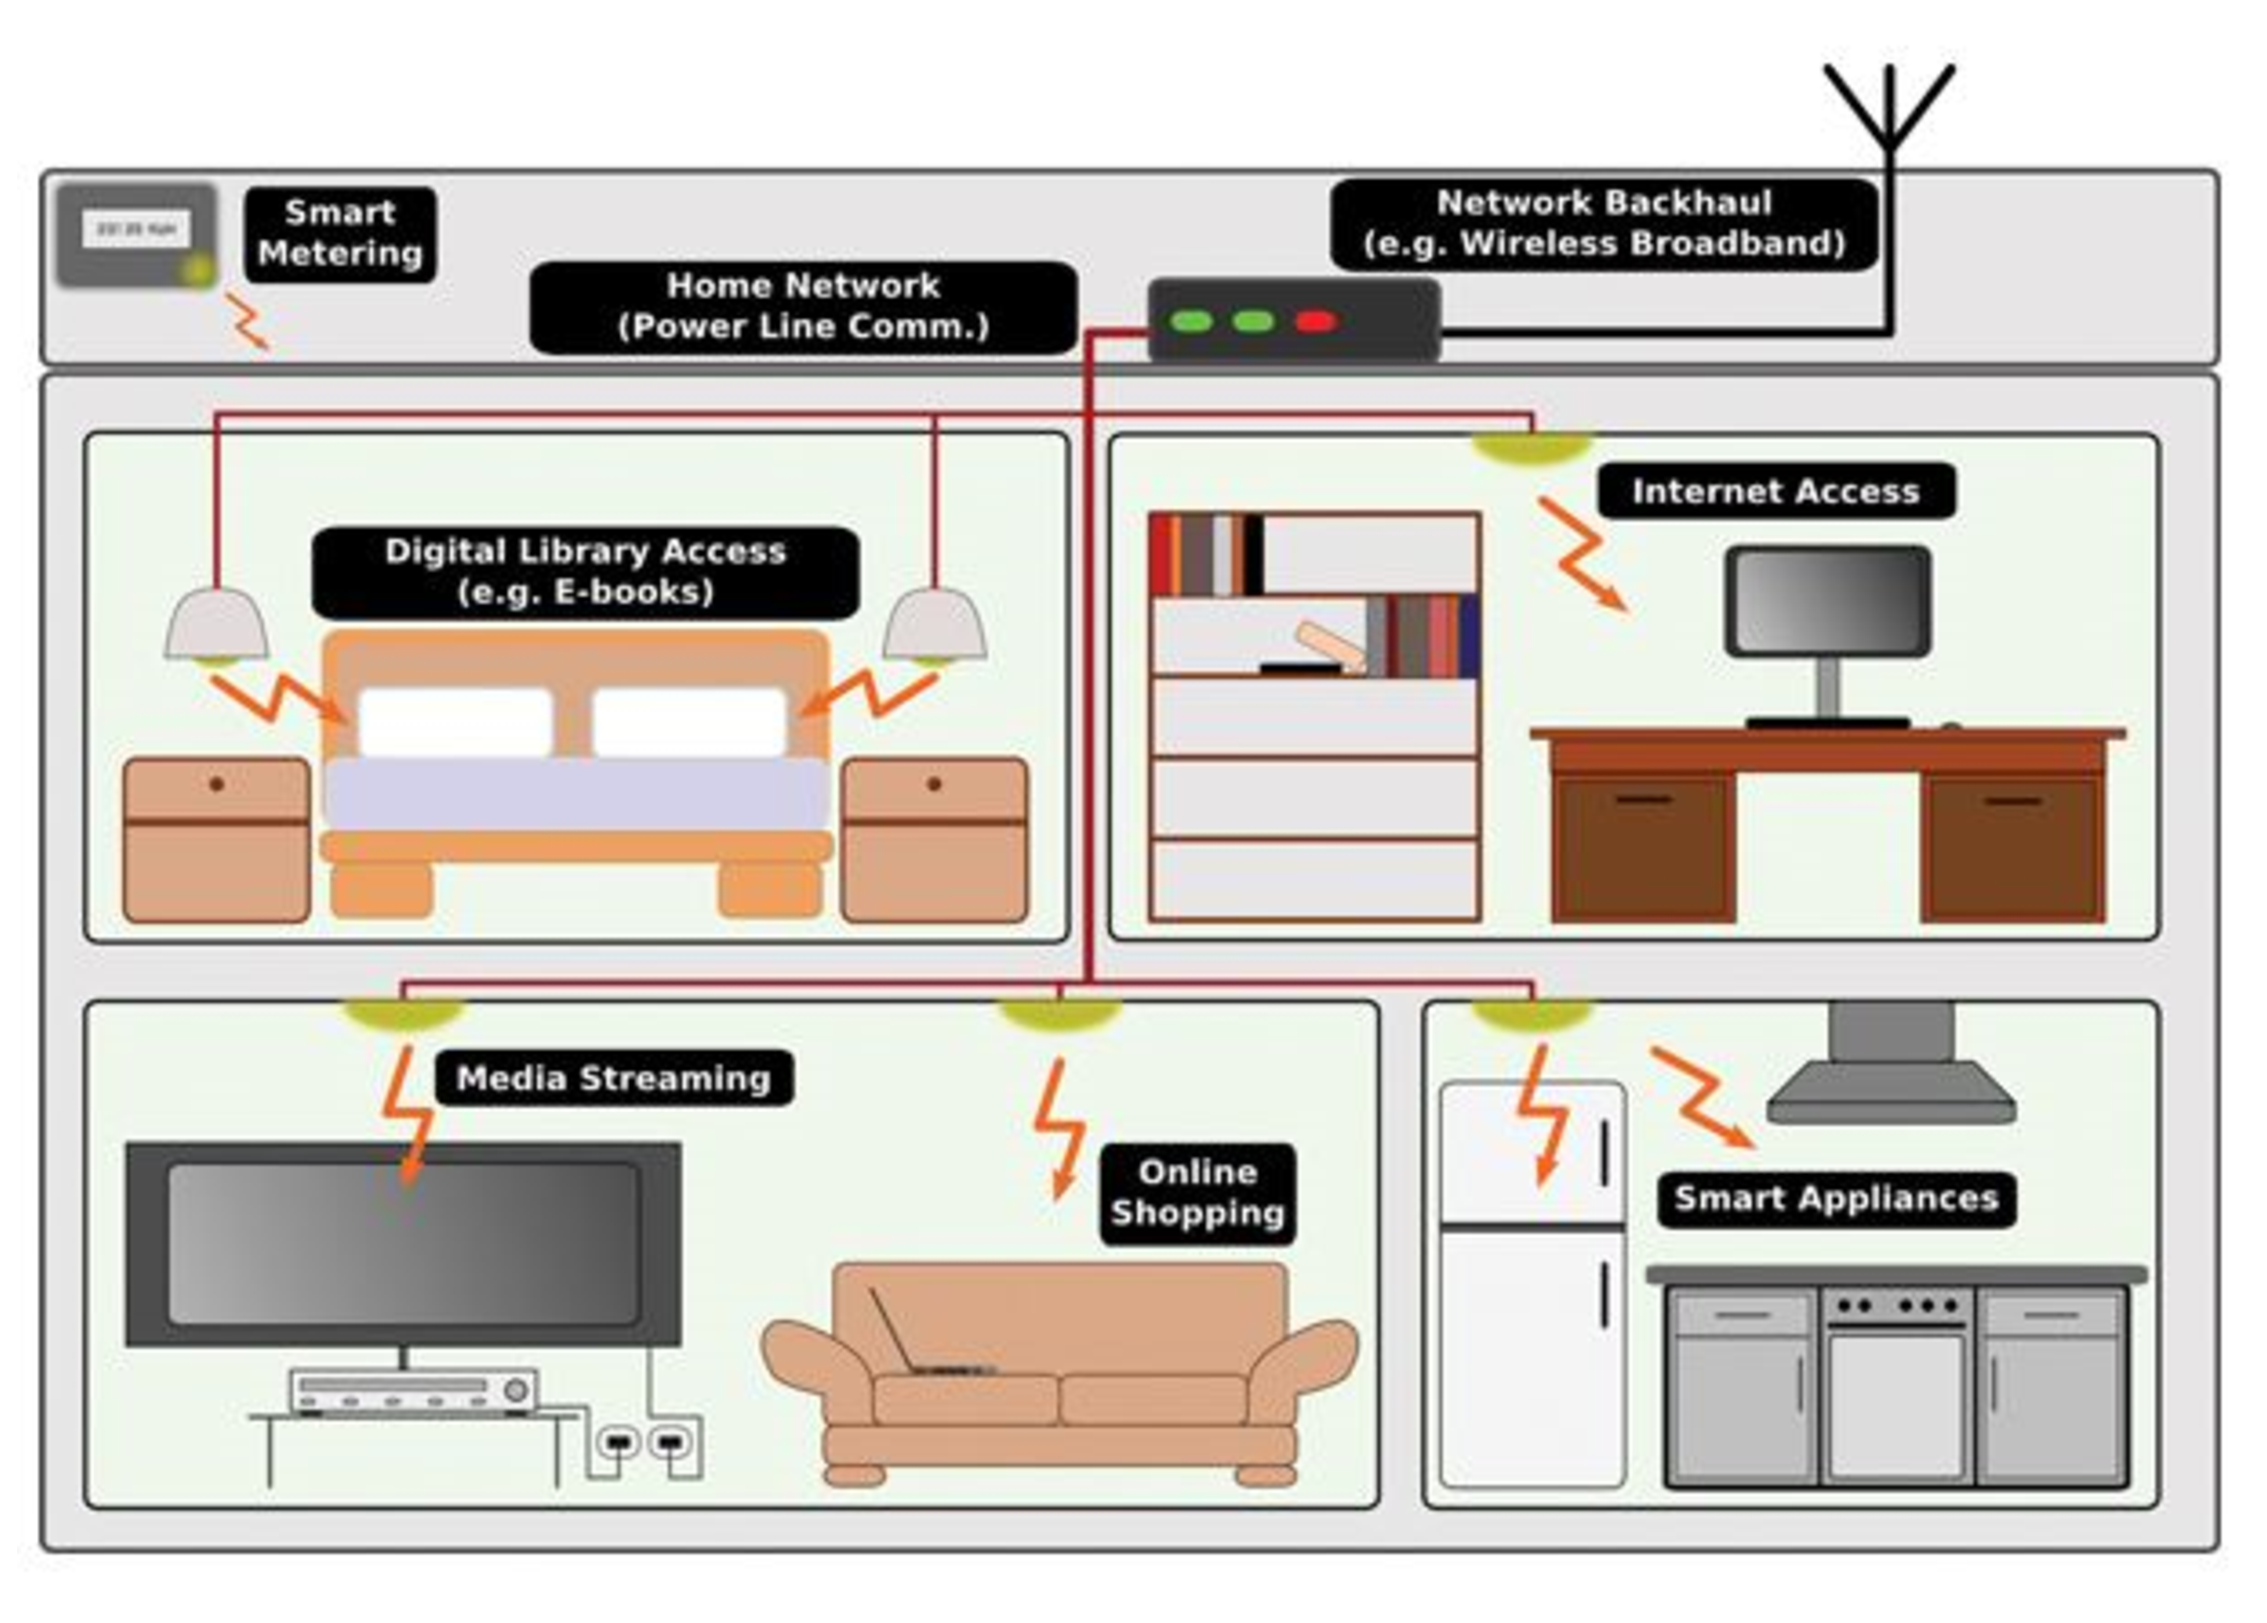
\includegraphics[width=4.5in]{basic1.eps}
%\caption{VLC Environment \cite{r19}.} \label{vlc}
%\end{center}
%\end{figure}
%%\pagebreak
%
%%This report is organized as follows:
%%
%%Chapter 1 includes about visible light communication history, spectrum analysis for VLC and characteristics of VLC. After this chapter 1 also discusses comparison between VLC and other technologies. Chapter 2 includes working technology of VLC. Chapter 3 provides the transmitter, channel and receiver required for VLC. Chapter 4 focuses on challenges for VLC. Chapter 5 is about modulation technique which are using in VLC and about standarisation for VLC. Chapter 6 includes various applications of VLC. Chapter 7 ends with an conclusion.
%
%
%\section{Visible light communication}
%
%\subsection {Brief history of Visible Light Communication.}
%The use of light to send messages is a very old idea. Fire and smoke signalling were used in ancient civilizations. For example, the ancient Greeks used polished shields to reflect sunlight to signal in the battle and Roman records indicate that polished metal plates were used as mirrors to reflect sunlight for long distance signalling. Chinese started using fire beacons followed by the Romans and American Indians using
%smoke signals.
%
%In the early 1800s, the US military used a wireless solar telegraph called “Heliograph” which is shown in figure that signals using
%Morse code flashes of sunlight reflected by a mirror. The flashes are produced by momentarily pivoting the mirror, or by interrupting the beam with a shutter. The diagram of heliograph is shown in Figure \ref{helio}. The navy often uses blinking lights, i.e. Aldis lamps, to
%send messages also using Morse code from one ship to another.
%\begin{figure}[h]
%\begin{center}
%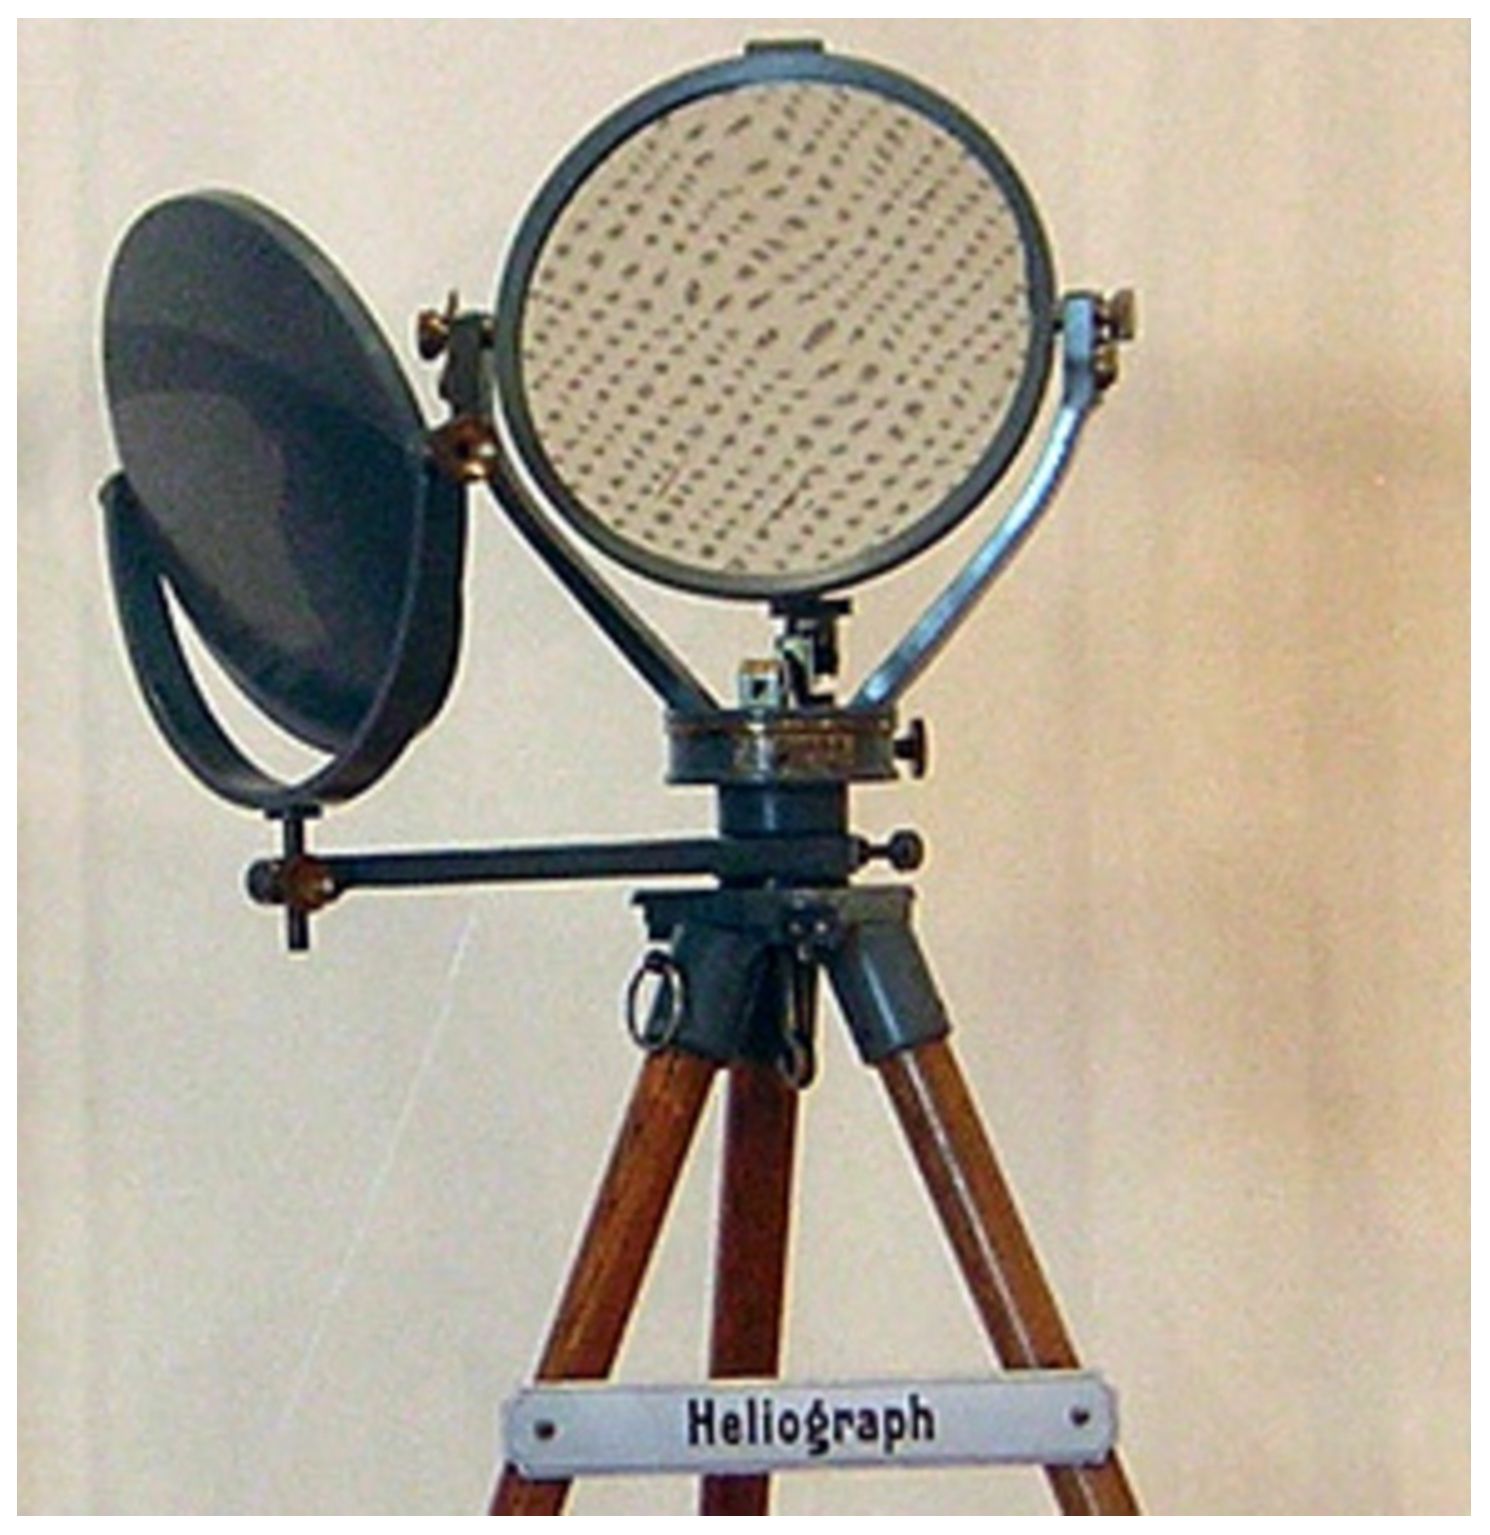
\includegraphics[width=3.0in]{heliograph.eps}
%\caption{Heliograph \cite{r17}.} \label{helio}
%\end{center}
%\end{figure}
%
%%\pagebreak
%
%In 1880, the first example of VLC technology was demonstrated by Alexander Graham Bell with his “photophone” that used sunlight
%reflected off a vibrating mirror and a selenium photo cell to send voice on a light beam. The transmitter and receiver of photophone is shown in Figure \ref{sun}.
%\begin{figure}[h]
%\begin{center}
%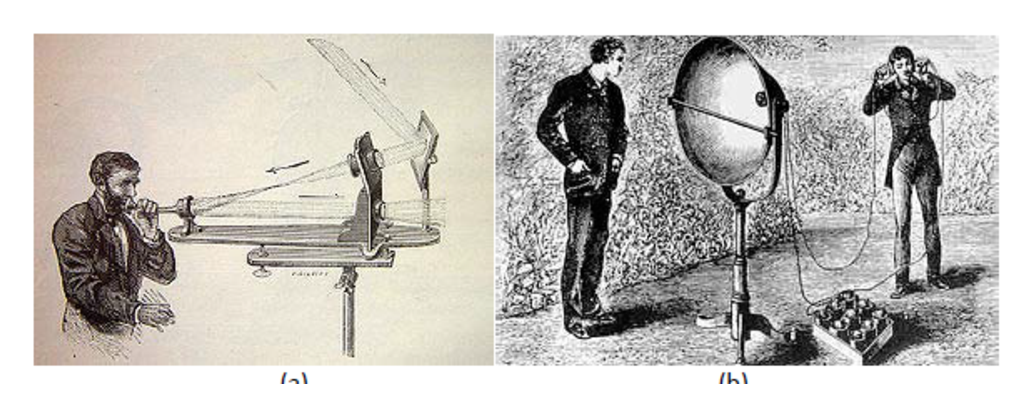
\includegraphics[width=4.0in]{sunlight.eps}
%\caption{(a) Photophone transmitter. (b) Photophone receiver and handset \cite{r17}.} \label{sun}
%\end{center}
%\end{figure}
%
%Until the late 1960s, radio and radar communications were more successful than optical communications
%(OC). OC started to get real attention with the invention of the light amplification by stimulated emission of
%radiation (laser) and the laser diode (LD) in the 1960s, followed in the 1970s by the development of lowloss
%optical fibres (OFs) as a medium for transmitting information using light, the invention of the OF amplifier in the 1980s, and the invention of the in-fibre Bragg grating in the 1990s. These inventions formed the basis for the telecommunications revolution of the late 20th century and provided the infrastructure for the Internet. The Nobel Prize in physics 2009 went to three scientists (Charles K. Kao, Willard S. Boyle,
%George E. Smith) who have played important roles in shaping the modern information technology due to
%their ground breaking achievements concerning the transmission of light in fibers for optical
%communication. Advancements in basic opto-electronic devices, such as LEDs (light emitting diodes) and
%LDs, p-intrinsic-n (PIN) photodiodes (PDs) and avalanche photo-diodes (APDs) and various optical
%components have attracted engineers to consider optical sources for wireless data transmission which has
%led to modern optical wireless communications (OWC) \cite{r17}.
%
%The first indoor OWC system was developed over 25 years ago. In 1979, an indoor OWC system was
%presented by Gfeller and Bapst. In their system, diffuse optical radiation in the near-IR region was
%utilised to interconnect a cluster of terminals located in a room to a common cluster controller.
%During the last ten years, we have witnessed the emergence of visible light communications (VLC) fuelled
%by solid-state lighting (SSL) technology. SSL is a rapidly developing area, both in terms of commercial
%exploitation, and academic and industrial research. LEDs with a wide range of colours are available,
%including white light. The output power as well as device efficiencies are increasing rapidly. The field of
%applications is also expanding. White LEDs are commonly used as replacements for incandescent lamps due
%to more than 10 times improved energy efficiency. Therefore, LED lighting is set to revolutionise the way
%we illuminate our homes, offices, public buildings and streets.
%
%These SSL sources, being semiconductor devices, come with an additional feature. Their light intensity can
%be varied at very high speeds, and so their functionality can be extended by means of intensity modulation
%(IM) to also become a wireless communication device.
%
%VLC originated in Japan and the visible light communications consortium (VLCC) was established in
%November 2003. The VLCC has major companies in Japan on board and aims at publicising and
%standardising VLC technology. The formation of the VLCC has stimulated worldwide interest in VLC
%technology, and the first IEEE standard for VLC - IEEE 802.15.7 – has emerged recently. University of
%Edinburgh academics have worked on VLC since 2004 and have developed enhanced modulation schemes
%that enable high data rates to be achieved using standard LED light bulbs.
%
%%%%%%%%%%%%%%%%%%%%%%%%%%%
%%The idea of using light as a communication medium was implemented by Alexander
%%Graham Bell in 1880 with his invention of the photophone, a device that transmitted a
%%voice signal on a beam of light. Bell focused sunlight with a mirror and then talked into a
%%mechanism that vibrated the mirror. The vibrating beam was picked up by the detector at
%%the receiving end and decoded back into the voice signal, the same procedure as the
%%phone did with electrical signals. But Bell could not generate a useful carrier frequency,
%%nor was he able to transmit the light beam from point to point. Obstacles in nature such as
%%fog and rain — which could interfere with the photophone — made Bell stop any future research into his invention [7]. With the invention of LED (Light Emitting Diode), the
%%idea of using light as a communication medium has started again. VLC uses white Light
%%Emitting Diodes (LED), which send data by flashing light at speeds undetectable to the
%%human eye. One major advantage of VLC is that we can use the infrastructure around us
%%without having to make any changes to it. LEDs’ ability to transfer information signals
%%over light ( light which is between 400THz to 800THz of frequency and whose
%%wavelength is between 400nm to 700nm ) makes it a very good communication medium.
%%Now the light we use in our daily life can not only be used for providing light but also for
%%communication.
%%%%%%%%%%%%%%%%%%%%%%%%%%%
%
%%Human being has used a visible light source as a form of data transmission since ancient
%%times.Since ancient times humans are using it in simple form. For example, in old times to give war signals, they used reflection of sunlight using brushed iron piece or smoke in day time and at night they were using fire to give signals. That was the best and very effective way to inform others by giving signal like this for that time as technology was not developed enough.
%
%%\begin{figure}[h]
%%\begin{center}
%%\includegraphics[width=4.0in]{history.eps}
%%\caption{Historical perspective of Visible Light Communications.} \label{his}
%%\end{center}
%%\end{figure}
%%
%%\begin{itemize}
%%  \item Sunlight
%%  The heliograph was used to send information over large distances by using reflecting
%%mirrors.
%%In 1880, Alexander Graham Bell invented the “Photophone”, which allowed
%%transmitting sounds over long distances on a beam of light. It is considered as the first
%%sophisticated wireless communications device.
%
%%\begin{figure}[h]
%%\begin{center}
%%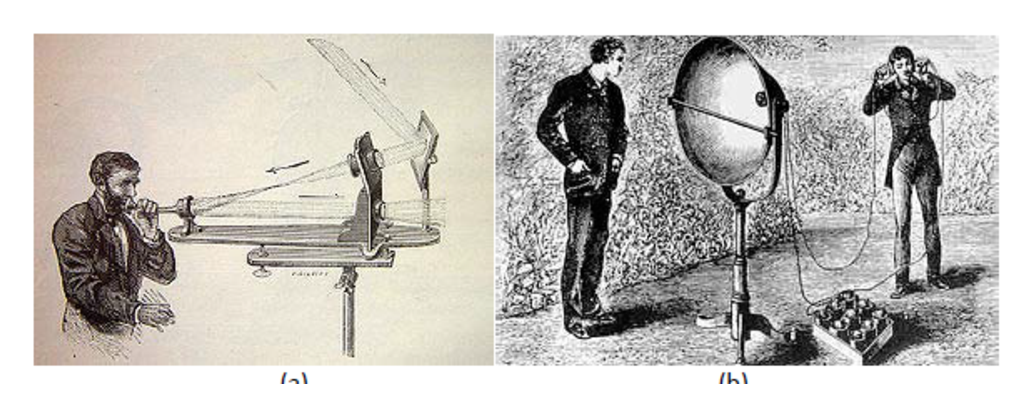
\includegraphics[width=4.0in]{sunlight.eps}
%%\caption{(a) Photophone transmitter. (b) Photophone receiver and handset.} \label{sun}
%%\end{center}
%%\end{figure}
%%\pagebreak
%%
%%  \item Fire
%%
%%  \item Lamps
%%
%%  \item LEDs
%
%%\end{itemize}
%
%\subsection {Spectrum Analysis}
%Since Visible light communication is a data communication technology that uses visible light between 380 nm and 780 nm. These wavelengths correspond to a frequency range of approximately 384 THz to 789 THz. In Figure \ref{mux} and \ref{vlc}, we can see a diagram of the visible light spectrum. The visible light spectrum is 10000 times larger than that of radio spectrum.	
%
%\begin{figure}[h]
%\begin{center}
%\includegraphics[width=4.0in]{spectrum.eps}
%\caption{Visible light portion in electromagnetic spectrum \cite{r17}.} \label{mux}
%\end{center}
%\end{figure}
%
%\begin{figure}[h]
%\begin{center}
%\includegraphics[width=4.0in]{vlcspectrum.eps}
%\caption{visible light spectrum \cite{r20}.} \label{vlc}
%\end{center}
%\end{figure}
%
%\pagebreak
%
%\subsection {Characteristics of VLC}
%
%The main characteristics of this technology are summarized below \cite{r1}:
%\begin{itemize}
%  \item Bandwidth :
%The bandwidth is virtually not limited, it offers a frequency band of  approximately 400THz.
%  \item Efficiency :
%VLC is highly energy efficient since illumination and transmission of data are done at the same time.
%  \item Data Rates :
%VLC can achieve high data rates (hundreds of Mb/s) and it can therefore be used for high speed wireless communications.
%  \item Cost :
%As VLC uses the visible light spectrum it is free of cost. Furthermore, transmitters and receivers are cheap.
%  \item Human Safety :
%VLC is harmless to human health and it is not injurious to the human eye.
%  \item Omnipresent Nature :
%We have the infrastructure because there are already a lot of LED-based lights installed in the world which are potential VLC transmitters and therefore we can use them for communications.
%  \item Security :
%As light waves do not penetrate opaque objects they can not  be intercepted, so it offers a very secure communication. It is very difficult for an intruder to make use of your signal.
%  \item Visibility :
%It is great to see data being communicated by a beam of light. What you see is what you send!
% % \item 
%\end{itemize}
%
%%This report is organized as follows:
%%
%%Chapter 1 includes about visible light communication history, spectrum analysis for VLC and characteristics of VLC. After this chapter 1 also discusses comparison between VLC and other technologies. Chapter 2 includes working technology of VLC. Chapter 3 provides the transmitter, channel and receiver required for VLC. Chapter 4 focuses on challenges for VLC. Chapter 5 is about modulation technique which are using in VLC and about standarisation for VLC. Chapter 6 includes various applications of VLC. Chapter 7 ends with an conclusion.
%
%
%%Traditiovnally, diggfital signal processing (DSP) algorithms are
%%implemented using general-purpose (programmable) D
%%in section \ref{organization},we haveeee further,subsection\ref{partt1}
%%\begin{tabular}{|c|c|}
%%                                                                         \hline
%%                                                                         % after \\: \hline or \cline{col1-col2} \cline{col3-col4} ...
%%                                                                         x & y \\
%%                                                                         1 & 2 \\
%%                                                                         \hline
%%                                                                       \end{tabular}
%
%%%%%%%%%%%%%%%%%%%%%%%
%%Chapter 1 of this thesis serves to provide an overview of the basic concepts and
%%techniques in physics and engineering and also shows several designs that are required
%%for the implementation of VLC. Chapter 2 provides the background needed for the VLC
%%designs. Chapter 3 provides the literature review of the VLC technology. Chapters 4 and
%%5 provide the experimental setup and implementation of the models. Chapter 6 presents
%%recommendations for improving the designs, as well as the conclusion with suggestions
%%for further improvements in the work.
%%%%%%%%%%%%%%%%%%%%%%
%%dbfvdjkhskjb lguuklrjkljknnn,mvn,n,nvkndknvkh
%%
%%\section{my section}
%%jhgfkjdhsjfhkjsdhkjghdfjkgkjhdfkjhsghfklhgjdfhgkjhfhghfklg
%%gfgbjsdbgjhjkfhjhgjsdkhjgjdhhkdjkghkdh
%%\subsection{gfhjdsh}
%%
%%my sub section is.
%
%
%
%%
%%\begin{figure}[h]
%%\begin{center}
%%%\includegraphics[width=4.0in]{creation-HD.eps}
%%\caption{The slab reactor.} \label{scenory}
%%\end{center}
%%\end{figure}
%%%
%%
%%\section{mdskjkjf}
%%jhbfjdhjk
%%\subsection{bbdbvjbdfj}
%%gvfkdnvknfk
%%\label{organization}
%%\label{SectionIntroduction}
%%\begin{tabular}{|c|c|}
%%  \hline
%%  % after \\: \hline or \cline{col1-col2} \cline{col3-col4} ...
%%  1 & 2 \\
%%  \hline
%%  3 & 4 \\
%%  \hline
%%\end{tabular}
%%
%%Digital filters are typically used to modify or alter the attributes
%%of a signal in the time or frequency domain. The most c
%%\subsection{part1}
%%\label{partt1}
%%]
%%%
%%\begin{eqnarray*}\label{eq0}
%%y(t)=\int_{\tau=0}^\infty\tau^2+\tan^3(\tau) \textmd{ } d\tau,
%%\end{eqnarray*}
%%%%
%%
%%In signal processing, the function of a filter is to remove unwanted
%%parts of the signal\cite{OPAgrawal_2_agrawal_defterli_baleanu}
%%
%%$\sin(x+y)$
%%
%%
%%
%%$\alpha_0$
%%
%%
%%
%%consider a number $x>2$ and $y<90$ such that $z=\sin(x+y)$.consider with$p=\sigma^2+\mu_3$.
%%%
%%\begin{eqnarray}\label{eq1}
%%35^{1035}&=&\sin(x+y)\\
%%x&=&y+z.
%%\end{eqnarray}
%%%%
%%\begin{table}
%%\caption{yoo yoo}
%%\begin{tabular}{|c|c|c|}
%%  \hline
%%  % after \\: \hline or \cline{col1-col2} \cline{col3-col4} ...
%%  \textbf{coloumn1} & 2 & 3 \\
%%  \hline
%%  e & f & fv \\
%%  \hline
%%  as & ss & ef \\
%%  \hline
%%\end{tabular}
%%\end{table}
%%\section{Organization of the report}
%%\begin{table}
%%\centering
%%\begin{tabular}{ c c c }
%%
%%  1 & 2 & 3 \\
%%  4 & 5 & 6 \\
%%  7 & 8 & 9 \\
%%\end{tabular}
%%\end{table}
%%Chapter 2 discusses the various ways of implementing the digital filter and tells that why fpga implementation is better compare to others.from equation(\ref{eq1}),we see \cite{FCBook_4_sabatier_agrawal_machado}
%%%
%%\begin{equation}\label{eq0}
%%\left[\begin{array}{c}
%%  1 \\
%%  2
%%\end{array}\right]=\left(
%%             \begin{array}{cc}
%%               1 & 3 \\
%%               0 & 2 \\
%%             \end{array}
%%           \right)\left[\begin{array}{c}
%%                    1 \\
%%                    2
%%                  \end{array}\right]
%%\end{equation}
%%%%
%%
%%chapter 3 discusses design stage for digital filter, which includes specification of
%%filter, calculation of filter coefficients, realization of filter structure, finite world length
%%effect and the design using windowing techniques are given in this chapter.
%%
%%
%%In Chapter 4, the Simulation and Synthesis tools which are used in implementation of
%%FIR filter is discussed. This chapter also discusses the FPGAs architecture, FPGA Design
%%Flow.
%%
%%
%%Chapter 5 discusses about how FIR filter can be realized and the process of
%%implementation of FIR filter. It also discusses restriction and assumption of filter,
%%choosing the filter structure, because it is often important to choose a particular filter
%%structure for a given transfer function H(z).This chapter also discusses Fixed Point
%%Representation of data.
%%
%%
%%
%%Chapter 6 contains results of simulation using  XILINX ISE 10.1i of
%%lowpass FIR filter.
%%
%%Chapter 7 concludes the project and also discusses future scope of work.
%\section{Comparison With Other Commuication Technologies}
%
%%%%%%%%%%%%%%%%%%%%%%%%%%%%%%%%%%%%%%%%%%%%%%%%%%%%%%%%%%%%%%%
%\subsection{Comparison with IR communication}
%
%The differences between VLC and infrared communication are listed in Table 1.
%
%%%%%%%%%%%%%%%%%%%%%%%%%%%%%%%%%%%%%%%%%%%%table
%\begin{table}[h]
%\caption{Comparison of short-range wireless communication technologies. (FIR: fast infrared, VFIR: very fast infrared) \cite{r15}.}
%\centering
%
%\begin{tabular}{|p{1in}|p{2in}|p{2in}|}
%%%\begin{tabular}{|c|c|c|}
%
%%\caption{Comparison of short-range wireless communication technologies (FIR fast infrared, VFIR very fast infrared).}
%  \hline
%  % after \\: \hline or \cline{col1-col2} \cline{col3-col4} ...
%  Parameters & Visible Light Communication & Infrared Communication \\
%  \hline
%  Data Rate & $>$100Mb/s possible (LED dependent)& 4Mb/s(FIR),16 Mb/s (VFIR) \\
%  \hline
%  Status & Research and standardization in IEEE & Standardization (IrDA) \\
%  \hline
%  Distance & ~meters & ~3 meters \\
%  \hline
%  Regulation & No & No \\
%  \hline
%  Security & Good & Good \\
%  \hline
%  Carrier wavelength (frequency) & 380$~$780 nm visible light (multiple wavelengths) & 850 nm infrared \\
%  \hline
%  Services & Communication, illumination & Communication \\
%  \hline
%  Noise Source & Sun light, Other illumination & Ambient light \\
%  \hline
%  Environmental & Daily usage Eye safe (visible) & Eye safe for low power (invisible) \\
%  \hline
%  Applications & Indoor vehicular communication, Optical ID & Remote control, Point to point connection \\
%  \hline
%\end{tabular}
%\label{table:comp}
%\end{table}
%
%%%%%%%%%%%%%%%%%%%%%%%%%%%%%%%%%%%%%%%%%%%%%%end table
%%\begin{tabular}{|c|c|}
%%  \hline
%%  % after \\: \hline or \cline{col1-col2} \cline{col3-col4} ...
%%  1 & 2 \\
%%  \hline
%%  3 & 4 \\
%%  \hline
%%\end{tabular}
%
%The infrared communication is standardized by the IrDA (Infrared Data Association) and
%the IrDA is still developing advanced application of infrared communication. The data rate
%for infrared communication (Knutson, 2004) includes 4 Mb/s (FIR), 16 Mb/s (VFIR), and etc.
%On the other hand, the VLC data rate is dependent on the LED’s modulation bandwidth and
%the standardization on physical layer specifications has not yet been published. Some of researches have reached around 20 Mb/s. Since the resonant-cavity LEDs shows the modulation bandwidth $>$ 100 Mb/s, it is expected that the VLC system with $>$ 100 Mb/s
%data rate is possible by using the high-speed LEDs and appropriate multiplexing techniques.
%
%The transmission distance for VLC is possible up to several meters due to its illumination
%requirement. Since the infrared communication is used for a remote controller, the
%maximum distance is ~ 3 meters. The VLC transmitter emits multiple-wavelength light from
%red to violet and the exact analysis will become more complex than infrared communication.
%
%Due to the wavelength of the light source, the noise sources will be different. For infrared
%communication, noise comes from ambient light containing infrared light. In the case of
%VLC, the sunlight and other illumination light can be noise sources. Also, the visible light is
%in our daily lives and we can detect it with human eye. Therefore, the VLC is eye safe.
%% The infrared communication has the long history and many applications have been developed
%%and are listed in (IrDA website). On the other hand, the VLC has shorter history and the
%%small number of applications has been proposed. Nevertheless, the illumination exists
%%everywhere and the VLC using the illumination infrastructure can be used easily.
%%By utilizing the characteristics of VLC link, it is expected to be candidate infrastructure for
%%indoor/outdoor public ubiquitous communication technology in the near future.
%%%%%%%%%%%%%%%%%%%%%%%%%%%%%%%%%%%%%%%%%%%%%%%%%%%%%%%%%%%%%%%%%%%%%%%5
%
%\subsection{Comparison with Radio Waves}
%Although radiofrequency communications is the most popular
%technology today, it also has disadvantages. VLC is compared
%with radiofrequency using five main concepts.
%\begin{itemize}
%  \item Capacity :
%  Radio spectrum is full and it is difficult to find radio
%capacity to support the demand of wireless data transmissions
%for media applications. The radio waves are limited, expensive
%and there is only a certain range of it. By using VLC more
%spectrums will be available and due to the infrastructure of
%LED-based lights installed in the world there is a potential for
%VLC as transmitters.
%  \item Efficiency :
%  Radio waves consume a lot of energy while VLC is
%highly energy efficient since illumination and transmission of
%data are done at the same time.
%  \item Cost :
%  VLC transmitters and receivers devices are cheap, there
%is no need for using expensive RF units.
%  \item Safety :
%  Radio wave creates Electromagnetic Interference
%(EMI), known to interfere with airplanes’ instruments and
%equipment in hospitals, and is potentially dangerous in
%hazardous operations, such as power/nuclear generation or oil
%and gas drilling. On the other hand, VLC uses light instead of
%radio waves, which is intrinsically safe and does not create
%EMI. Hence, this technology can be used in many places.
%  \item Security :
%  Radio waves penetrate through walls and they can be
%intercepted. By using VLC data is transmitted where the light is
%because light does not penetrate through walls, that is to say,
%VLC provide a secure data communication.
%\item Human Health :
%The transmission power of radio waves van
%cannot be increased over a certain level because there are
%serious health risks for humans. VLC is an attractive candidate
%in a consumer communication system.
%\end{itemize}
%
%This report is organized as follows:
%
%Chapter 1 includes about visible light communication history, spectrum analysis for VLC, characteristics of VLC along with comparison between VLC and other technologies. Chapter 2 includes working technology of VLC. Chapter 3 provides an explanation for the transmitter, channel and receiver required for VLC. Chapter 4 focuses on challenges for VLC. Chapter 5 is about modulation technique which are used in VLC and about standarisation for VLC. Chapter 6 includes various applications of VLC. Chapter 7 ends with an conclusion.             % Chapter 1: Introduction
\chapter{Literature Survey}

Traditiovnally, diggfital signal processing (DSP) algorithms are
implemented using general-purpose (programmable) D
in section \ref{organization},we haveeee further,subsection\ref{partt1}
\begin{tabular}{|c|c|}
                                                                         \hline
                                                                         % after \\: \hline or \cline{col1-col2} \cline{col3-col4} ...
                                                                         x & y \\
                                                                         1 & 2 \\
                                                                         \hline
                                                                       \end{tabular}
                   % Other chapters as required
%\include{chap_conclusions}      % Finally the summary & conclusions

%--------------------------------------------------------------------%
% APPENDIX
%  Appendices, if any, must precede the cited literatures.
%  Appendices shall be numbered in Roman Capitals (e.g. Appendix IV)
\appendix
%\include{appendix_1}        % Appendices if any..

%--------------------------------------------------------------------%
% LITERATURE CITED
%   This should follow the appendices, if any, otherwise summary and
%   conclusions chapter.
\bibliography{xyz}              % Make the bibliography

%--------------------------------------------------------------------%
% ACKNOWLEDGMENTS
%   For APS, acknowledgements can be the first item after title page
%      OR
%   the very last item.
%
\begin{acknowledgments}
I thank the many people who have done lots of nice things for me.
\end{acknowledgments}


\end{document}
